\documentclass{tufte-handout}

\title{Discrete Probabilistic Programming Languages III: Observation \& Sampling\thanks{CS7470 Fall 2023: Foundations of Probabilistic Programming.}}


\newcommand{\varset}[0]{\mathcal{V}}

\author[]{Steven Holtzen\\s.holtzen@northeastern.edu}

%\date{28 March 2010} % without \date command, current date is supplied

%\geometry{showframe} % display margins for debugging page layout
\setcounter{secnumdepth}{1}

\usepackage{graphicx} % allow embedded images
  \setkeys{Gin}{width=\linewidth,totalheight=\textheight,keepaspectratio}
  \graphicspath{{graphics/}} % set of paths to search for images
\usepackage{amsmath,amssymb,amsthm}  % extended mathematics
\usepackage{booktabs} % book-quality tables
\usepackage{units}    % non-stacked fractions and better unit spacing
\usepackage{multicol} % multiple column layout facilities
\usepackage{lipsum}   % filler text
\usepackage{fancyvrb} % extended verbatim environments
  \fvset{fontsize=\normalsize}% default font size for fancy-verbatim environments
\usepackage{listings}
\usepackage{tikz}
\usepackage{mathpartir}
\usepackage{subcaption}
\usepackage{mdframed}
\usepackage{epigraph}
\usepackage{enumitem}
\usepackage{stmaryrd}

\usetikzlibrary{shapes.geometric}


\usepackage[ruled,linesnumbered]{algorithm2e}
\SetKwComment{Comment}{/* }{ */}
\newcommand{\indep}{\perp \!\!\! \perp}

\tikzset{
  treenode/.style = {shape=rectangle, rounded corners,
                     draw, align=center,
                     },
  root/.style     = {treenode, font=\Large, bottom color=red!30},
  env/.style      = {treenode, font=\ttfamily\normalsize},
  dummy/.style    = {circle,draw}
}

% tikz
\usetikzlibrary{patterns,calc,backgrounds}


% TIKZ
\tikzstyle{nnf}=[
  >=stealth,font=\small,auto,scale=0.7,every node/.style={scale=0.7}
]
\tikzstyle{extnode}=[
  draw,circle,inner sep=2pt,fill=white
]

\tikzstyle{leafnode}=[
  draw,fill=gray!20,inner sep=3.5pt
]
\tikzstyle{constnode}=[
  draw,fill=white,inner sep=3.5pt
]
\tikzstyle{label}=[
  fill=white,inner sep=2.5pt
]

\tikzstyle{acarrow}=[
    decoration={markings,mark=at position 1 with {\arrow[scale=0.6]{>}}},
    postaction={decorate},
    shorten >=0.4pt,
    >=latex,
    line width=0.1
]

\tikzstyle{bnarrow}=[
    decoration={markings,mark=at position 1 with {\arrow[scale=1.5]{>}}},
    postaction={decorate},
    shorten >=0.7pt,
    >=latex,
    line width=0.3
]
\tikzstyle{bayesnet}=[
  >=latex, thick, auto
]
\tikzstyle{bnnode}=[
  draw,ellipse,minimum size=7mm,inner sep=1pt,font=\small
]
\tikzstyle{cpt}=[
  font=\footnotesize
]

\tikzstyle{graph}=[
  >=stealth,font=\small,auto,scale=1,every node/.style={scale=1}
]
\tikzstyle{node}=[
  draw,circle,inner sep=3pt,fill=white
]

% BDDs

\tikzstyle{bdd}=[
  >=latex, thick, >=stealth, font=\small,auto,scale=0.9,every node/.style={scale=0.9}
]
\tikzstyle{bddnode}=[
  draw,circle,inner sep=0pt,fill=white,minimum size=5.5mm
]

\tikzstyle{bddtriangle}=[
  draw, regular polygon, regular polygon sides = 3,inner sep=1pt,fill=white,minimum size=5.5mm
]

\tikzstyle{highedge}=[
    line width=0.9
]
\tikzstyle{lowedge}=[
    line width=0.9,dotted
]
\tikzstyle{bddterminal}=[
  draw,fill=gray!20,inner sep=2.5pt, font=\small
]

\lstdefinestyle{compact}{
  \ttfamily\tiny
}


\usetikzlibrary{positioning}

\newtheorem{theorem}{Theorem}
\newtheorem{definition}{Definition}
\newtheorem{conjecture}{Conjecture}
\newtheorem{lemma}{Lemma}
\newtheorem{exercise}{Exercise}
\newtheorem{remark}{Remark}


\usepackage{xcolor}

\definecolor{codegreen}{rgb}{0,0.6,0}
\definecolor{codegray}{rgb}{0.5,0.5,0.5}
\definecolor{codepurple}{rgb}{0.58,0,0.82}
\definecolor{backcolour}{rgb}{0.95,0.95,0.92}

\lstdefinestyle{mystyle}{
    backgroundcolor=\color{backcolour},   
    commentstyle=\color{codegreen},
    keywordstyle=\color{magenta},
    numberstyle=\tiny\color{codegray},
    stringstyle=\color{codepurple},
    basicstyle=\ttfamily\footnotesize,
    breakatwhitespace=false,         
    breaklines=true,                 
    captionpos=b,                    
    keepspaces=true,                 
    numbers=left,                    
    numbersep=5pt,                  
    showspaces=false,                
    showstringspaces=false,
    showtabs=false,                  
    tabsize=2
}

\lstset{style=mystyle}

\newcommand{\defn}[1]{\textbf{#1}}
\newcommand{\dbracket}[1]{\left \llbracket {#1} \right \rrbracket}
\newcommand{\dist}[1]{\mathtt{Dist}(#1)}
\newcommand{\true}[0]{\texttt{true}}
\newcommand{\te}[0]{\texttt{e}}
\newcommand{\false}[0]{\texttt{false}}
\newcommand{\real}[0]{\mathbb{R}}
\newcommand{\rational}[0]{\mathbb{Q}}
\newcommand{\lebesgue}[0]{\mathbb{L}}
\newcommand{\eval}[0]{\mathrm{ev}}
\newcommand{\disc}[0]{\textsc{Disc}}
\newcommand{\borel}[0]{\mathcal{B}}
\newcommand{\ent}[0]{\mathbb{S}}
\newcommand{\prog}[0]{\texttt{p}}
\newcommand{\bool}[0]{\mathbb{B}}
\newcommand{\cont}[0]{\textsc{Cont}}
\newcommand{\prop}[0]{\textsc{Prop}}
\newcommand{\bdd}[0]{\textsc{Bdd}}
\newcommand{\robdd}[0]{\textsc{Robdd}}
\newcommand{\compiles}[0]{\rightsquigarrow}

\newcommand{\bddtriangle}[1]{
    \begin{tikzpicture}
    \node [bddtriangle] {#1};
    \end{tikzpicture}}
\newcommand{\bddtrue}[0]{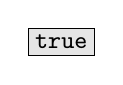
\begin{tikzpicture}
      \node [bddterminal] {$\true$};
    \end{tikzpicture}}
\newcommand{\bddfalse}[0]{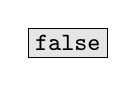
\begin{tikzpicture}
      \node [bddterminal] {$\false$};
    \end{tikzpicture}}


% Standardize command font styles and environments
\newcommand{\doccmd}[1]{\texttt{\textbackslash#1}}% command name -- adds backslash automatically
\newcommand{\docopt}[1]{\ensuremath{\langle}\textrm{\textit{#1}}\ensuremath{\rangle}}% optional command argument
\newcommand{\docarg}[1]{\textrm{\textit{#1}}}% (required) command argument
\newcommand{\docenv}[1]{\textsf{#1}}% environment name
\newcommand{\docpkg}[1]{\texttt{#1}}% package name
\newcommand{\doccls}[1]{\texttt{#1}}% document class name
\newcommand{\docclsopt}[1]{\texttt{#1}}% document class option name
\newenvironment{docspec}{\begin{quote}\noindent}{\end{quote}}% command specification environment



\begin{document}
\maketitle% this prints the handout title, author, and date

\section{Observation}
\begin{itemize}
  \item Why observation? 
  \item \texttt{observe} is a powerful keyword that lets us \emph{condition} the
program. For instance, suppose I want to model the following scenario: ``flip 
two coins and observe that at least one of them is heads. What is the probability 
that the first coin was heads?''

We can encode this scenario as a \disc{} program:

\begin{lstlisting}[mathescape=true, caption={\textsc{TwoCoins}}]
x $\leftarrow$ flip 0.5; 
y $\leftarrow$ flip 0.5;
observe x $\lor$ y;
return x
\end{lstlisting}

This program outputs the probability distribution:
\begin{align*}
  [\true \mapsto (0.25 + 0.25) / 0.75, \false
\mapsto 0.25 / 0.75]
\end{align*} 

\item Denotational semantics of \texttt{observe}:
  \begin{align*}
  \dbracket{\texttt{observe}~\te_1; \te_2]}(v) = 
  \sum_{\{v' \mid \dbracket{e_1}(v') = T\}} \dbracket{\te_2}(v)
  \end{align*}

  Note that, with this definition, the semantics of probabilistic terms are now
  \emph{unnormalized} (i.e., the distribution does not sum to 1). For example:
  \begin{align*}
    \dbracket{\false} = \begin{cases}
      \true &\mapsto 0 \\ 
      \false &\mapsto 0
    \end{cases}
  \end{align*}

  The \textsc{TwoCoins} case:
  \begin{align*}
    \dbracket{\textsc{TwoCoins}} = \begin{cases}
      \true &\mapsto 0.5 \\ 
      \false &\mapsto 0.25
    \end{cases}
  \end{align*}
  

\item  The main semantic object of interest is 
the \emph{normalized distribution}, which is given by the \defn{normalized semantics}:
\begin{align*}
\dbracket{\te}_D(T) = \frac{\dbracket{\te}(T)}{\dbracket{\te}(T) + \dbracket{\te}(F) },
\end{align*}


defined analogously for the false case.
  \item In order to handle observations, we will compile \disc{} programs into 
  \emph{two} \prop{} programs: one that computes the unnormalized probability of 
  returning $\true$, and one that computes the probability of evidence (i.e. normalizing constant)
  \item Inductive description has the shape $\te \compiles (\texttt{p}_1, \texttt{p}_2)$. 

  Our goal will be for this compilation to satisfy the following form of semantics-presevation:
  \begin{theorem}[Semantics preservation]
    For well-typed closed term $\te$,
    assume $\te \compiles (\varphi, \varphi_A, w)$. Then, 
    $\dbracket{\te}_D(\true) = {\dbracket{(\varphi \land \varphi_A, w)}} / {\dbracket{(\varphi_A, w)}}$.
  \end{theorem}

  \item Compilation relation:
  \begin{mathpar}
    \inferrule{}{\true \compiles (\true, \true, \emptyset)} \and 
    \inferrule{}{\false \compiles (\false, \true, \emptyset)} \and 
    \inferrule{}{x \compiles (x, \true, \emptyset)} \and 
    \inferrule{\texttt{fresh}~x}
      {\texttt{flip}~\theta \compiles (x, \true, [x \mapsto \theta, \overline{x} \mapsto 1-\theta])} \and
    \inferrule{\te_1 \compiles (\varphi, \varphi_A, w) \and \te_2 \compiles (\varphi', \varphi_A', w')}
      {x \leftarrow \te_1; \te_2 \compiles (\varphi'[\varphi/x], \varphi_A'[\varphi/x] \land \varphi_A, w_1 \cup w_2)} \and
    \inferrule{\te_1 \compiles (\varphi, \true, \emptyset) \and \te_2 \compiles (\varphi', \varphi_A', w)}
      {\texttt{observe}~\te_1; \te_2 \compiles (\varphi', \varphi \land \varphi_A', w)}
  \end{mathpar}

  Most of these rules are unchanged from the previous compilation, except for bind and \texttt{observe}.

  \item Example derivation:
  
  \begin{mathpar}
    \inferrule{\texttt{flip}~\theta \compiles (f, \true, [f \mapsto 1/2, \overline{f} \mapsto 1/2]) \and 
      \inferrule{x \compiles (x, \true, \emptyset) 
      \and 
      \inferrule{x \compiles (x, \true, \emptyset)}{\texttt{return}~x \compiles (x, \true, \emptyset)}}
      {\texttt{observe}~x; \texttt{return}~x \compiles (x, x, \emptyset)}
    }
      {x \leftarrow \texttt{flip}~\theta;~\texttt{observe}~x; \texttt{return}~x \compiles (f, f, [f \mapsto 1/2, \overline{f} \mapsto 1/2])}
  \end{mathpar}

  Check that this satisfies semantics preservation.

\end{itemize}

\section{Some notes on the project}
\begin{itemize}
  \item Instead of compiling to Prop, you can work directly on the BDD
  \item The basic primitive operation you will perform on BDDs is \emph{weighted
  model counting}, which is a more general term for what we've so far calling 
  the semantics of \textsc{Prop}:
  \begin{definition}[Weighted model count]
    Let $\varphi$ be a propositional formula and $w$ be a map from literals
    (assignments to variables) to real-valued weights. The \emph{weighted model count}
    is defined:
    \begin{align}
      \mathtt{WMC}(\varphi,w) \triangleq \sum_{I \models \varphi} \prod_{\ell \in I} w(\ell).
    \end{align}
  \end{definition}
  You can see an example of running a weighted model count in \texttt{disc/lib/kc.ml}
\end{itemize}

% \begin{theorem}
% Assume $\Gamma \vdash \te$ and $\te \compiles \prog$. Then, for any substitution
% $\gamma \in \dbracket{\Gamma}$, is is the case that 
% $\dbracket{\te[\gamma]}_D(\true) = \dbracket{\prog[\gamma]}$.
% \end{theorem}


\section{Sampling \& approximate reasoning}
\begin{itemize}
  \item Up until now we have been exclusively discussing \emph{exact reasoning}:
  computing the exact probability that a program will output a particular value

  \item Problems with exact reasoning:
  \begin{itemize}
    \item State-space explosion
    \item Limited expressive power: how can we handle continuous probability, or loops that may never terminate?
    \item ``All-or-nothing'': exact answer or nothing at all
  \end{itemize}

  \item An alternative is \emph{approximate reasoning}. Many of the most popular PPLs in use 
  today support exclusively this mode of reasoning.\sidenote{For example, Stan~\citep{carpenter2017stan}.}

  \item There is an entirely separate school of PPLs that reason by \emph{sampling}.

  \item The crucial mechanism is the \emph{sample mean}, which gives an estimate of the expectation 
  of a random variable:
  
  \begin{definition}[Expectation]
    Let $(\Omega, \Pr)$ be a probability space and $f : \Omega \rightarrow
    \real$ be a random variable. The \emph{expectation} (or \emph{average value}) of $f$ with respect to 
    $\Pr$ is defined:
    \begin{align}
      \E_{\Pr[f]} \triangleq \sum_{\omega \in \Omega} \Pr(\omega) f(\omega).
    \end{align}
  \end{definition}

  \begin{definition}[Sample mean]
    Let $(\Omega, \Pr)$ be a probability space and $f : \Omega \rightarrow
    \real$ be a random variable. Then, the \emph{sample mean} of $f$ 
    with $N$ samples is defined:
    \begin{align}
      \frac{1}{N} \sum_{\omega_i \sim \Pr}^N f(\omega_i),
    \end{align}
    where the notation $\omega_i \sim \Pr$ denotes drawing a sample $\omega_i$ from 
    the probability distribution $\Pr$.
  \end{definition}

  \marginnote{One may wonder \emph{how quickly} a particular
  estimate of the mean approaches the true value (i.e., how many samples one
  must draw in order to have an accurate estimate with high probability). There
  are many bounds of this sort known broadly as \emph{concentration
  inequalities}; \citet{shalev2014understanding} has a nice summary of some 
  of the useful concentration inequalities that arise in practice in the appendix.}

  \item The reason why we use the sample estimator is that the \emph{law of large numbers} 
  guarantees that, as $N \rightarrow \infty$, the sample mean approaches the 
  expectation, i.e.:
  \begin{align}
    \lim_{N \rightarrow \infty} \frac{1}{N} \sum_{\omega_i \sim \Pr}^N f(\omega_i) = \E_{\Pr}[f].
  \end{align}

  \item What will do is give a semantics to programs in terms of expectations, and then 
  use the expectation estimator in order to get an approximation for the program's 
  behavior

\end{itemize}


\bibliographystyle{plainnat}
\bibliography{../bib}


\end{document}